% !TEX program = pdflatex
\documentclass[12pt,a4paper]{article}

% -------------------------------------------------
% Packages
% -------------------------------------------------
\usepackage[a4paper,margin=1in]{geometry}
\usepackage[T1]{fontenc}
\usepackage[utf8]{inputenc}
\usepackage[expansion=false]{microtype}
\usepackage{setspace}
\usepackage{parskip}
\usepackage{titlesec}
\usepackage{xcolor}
\usepackage{listings}
\usepackage{fancyhdr}
\usepackage{lastpage}
\usepackage{enumitem}
\usepackage{booktabs}
\usepackage{array}
\usepackage{hyperref}
\usepackage{graphicx}

% -------------------------------------------------
% General formatting
% -------------------------------------------------
\onehalfspacing
\setlength{\parindent}{0pt}

\hypersetup{
    colorlinks=true,
    linkcolor=black,
    urlcolor=blue,
    pdftitle={Blockchain Laboratory - Experiment 3},
    pdfauthor={}
}

\pagestyle{fancy}
\fancyhf{}
\lhead{Blockchain Laboratory}
\rhead{Experiment No. 3}
\cfoot{Page \thepage}
\setlength{\headheight}{15pt}

\titleformat{\section}
  {\large\bfseries}
  {\thesection.}
  {0.5em}
  {}
\titleformat{\subsection}
  {\normalsize\bfseries}
  {\thesubsection.}
  {0.5em}
  {}

% -------------------------------------------------
% Code formatting
% -------------------------------------------------
\definecolor{codebg}{RGB}{248,248,248}
\definecolor{codecomment}{RGB}{80,120,80}
\definecolor{codekeyword}{RGB}{70,70,150}
\definecolor{codestring}{RGB}{150,70,70}

\lstdefinestyle{pythonstyle}{
    language=Python,
    backgroundcolor=\color{codebg},
    basicstyle=\ttfamily\footnotesize,
    keywordstyle=\color{codekeyword}\bfseries,
    commentstyle=\color{codecomment},
    stringstyle=\color{codestring},
    numbers=left,
    numberstyle=\tiny\color{gray},
    numbersep=8pt,
    frame=single,
    framerule=0.4pt,
    breaklines=true,
    breakatwhitespace=false,
    showstringspaces=false,
    tabsize=4,
    columns=fullflexible,
    keepspaces=true,
    literate={→}{{$\rightarrow$}}1
}

% -------------------------------------------------
% Document
% -------------------------------------------------
\begin{document}

% -------------------------------------------------
% Title page
% -------------------------------------------------
\begin{titlepage}
    \centering
    \vspace*{1.5cm}

    {\Large\bfseries BLOCKCHAIN LABORATORY\par}
    \vspace{1.2cm}

    {\large\bfseries Experiment No. 3\par}
    \vspace{0.8cm}

    {\LARGE\bfseries Create a Cryptocurrency using Python\par}

    \vspace{1cm}

    \begin{tabular}{rl}
    \textbf{Name:} & Nikhil Sunchu \\[0.6cm]
    \textbf{Roll No.:} & 31 \\[0.6cm]
    \textbf{Class/section} & D20A \\[0.6cm]
    \textbf{Date}& \hrulefill \\[0.6cm]
    \end{tabular}

    \vfill
    {\large Blockchain Laboratory\par}
\end{titlepage}

% -------------------------------------------------
\section{Aim}
Create a Cryptocurrency using Python and perform mining in the Blockchain created.

% -------------------------------------------------
\section{Theory}

\subsection{1. Blockchain Overview}
Blockchain is a distributed and decentralized ledger that stores information in a series of linked blocks. Each block contains transaction data, a timestamp, the previous block's hash, and its own unique hash (a digital fingerprint). Once data is recorded, it becomes immutable, because altering one block would require recalculating all subsequent blocks.

\subsection{2. Mining}
Mining is the process of collecting pending transactions into a block, solving a computational puzzle (Proof-of-Work) to find a valid hash, and adding the new block to the blockchain before broadcasting it to all connected peers. Miners are rewarded with cryptocurrency for successfully mining a block.

\subsection{3. Multi-Node Blockchain Network}
In this lab we simulate three independent blockchain nodes running on ports 5001, 5002, and 5003. Each node runs on a separate port, maintains its own copy of the blockchain, and can connect with peers to share and validate blocks.

\subsection{4. Consensus Mechanism}
We use the \emph{Longest Chain Rule}: if multiple versions of the chain exist, the longest valid chain is chosen. This ensures that all nodes agree on a single transaction history.

\subsection{5. Transactions and Mining Reward}
Each transaction has a sender, a receiver, and an amount. When a block is mined, the pending transactions are added to the block, and a reward transaction is added automatically to pay the miner.

\subsection{6. Chain Replacement}
When \texttt{/replace\_chain} is called, the node requests the chains from all its peers. If it finds a longer and valid chain, it replaces its own chain with it, keeping the blockchain consistent across all nodes.

% -------------------------------------------------
\section{Tools and Libraries Used}
\begin{itemize}
    \item Python 3.x
    \item Flask -- web framework for the API endpoints (\texttt{pip install Flask})
    \item Requests -- HTTP communication between nodes (\texttt{pip install requests==2.18.4})
    \item Postman -- for testing the API requests
    \item Python standard libraries: \texttt{datetime}, \texttt{jsonify}, \texttt{hashlib}, \texttt{uuid4}, \texttt{urlparse}, \texttt{request}
\end{itemize}

% -------------------------------------------------
\section{Tasks Performed}

\subsection{Task 1 -- Download the Code}
The files \texttt{hadcoin\_node\_5001.py}, \texttt{hadcoin\_node\_5002.py}, and \texttt{hadcoin\_node\_5003.py} were downloaded. Each implements a full cryptocurrency node -- the \texttt{Blockchain} class plus a Flask API -- differing only in the port number and the mining-reward receiver name.

\subsection{Task 2 -- Install the Required Packages}
The \texttt{requests} library was installed in the virtual environment created in Lab 2, together with \texttt{Flask}:
{\renewcommand{\baselinestretch}{0.85}\selectfont
\begin{lstlisting}[style=pythonstyle, numbers=none]
pip install Flask
pip install requests==2.18.4
\end{lstlisting}
}

\subsection{Task 3 -- Run the Three Nodes in Separate Terminals}
The three node files were run in three separate terminals, so each node listens on its own port (5001, 5002, 5003) and maintains its own copy of the blockchain.

\subsection{Task 4 -- Connect the Nodes (POST /connect\_node)}
The peers were registered from each node by invoking \texttt{connect\_node()} with a POST request containing the node addresses in JSON. \texttt{add\_node()} parses each URL with \texttt{urlparse()} and stores the network location (e.g.\ \texttt{127.0.0.1:5002}) in the node set.

{\renewcommand{\baselinestretch}{0.85}\selectfont
\begin{lstlisting}[style=pythonstyle]
def add_node(self, address):
    parsed_url = urlparse(address)
    self.nodes.add(parsed_url.netloc)

@app.route('/connect_node', methods=['POST'])
def connect_node():
    json = request.get_json()
    nodes = json.get('nodes')
    if nodes is None:
        return 'No node', 400
    for node in nodes:
        blockchain.add_node(node)
    return jsonify({'message': 'All the nodes are now connected.',
                    'total_nodes': list(blockchain.nodes)}), 201
\end{lstlisting}
}

\begin{center}
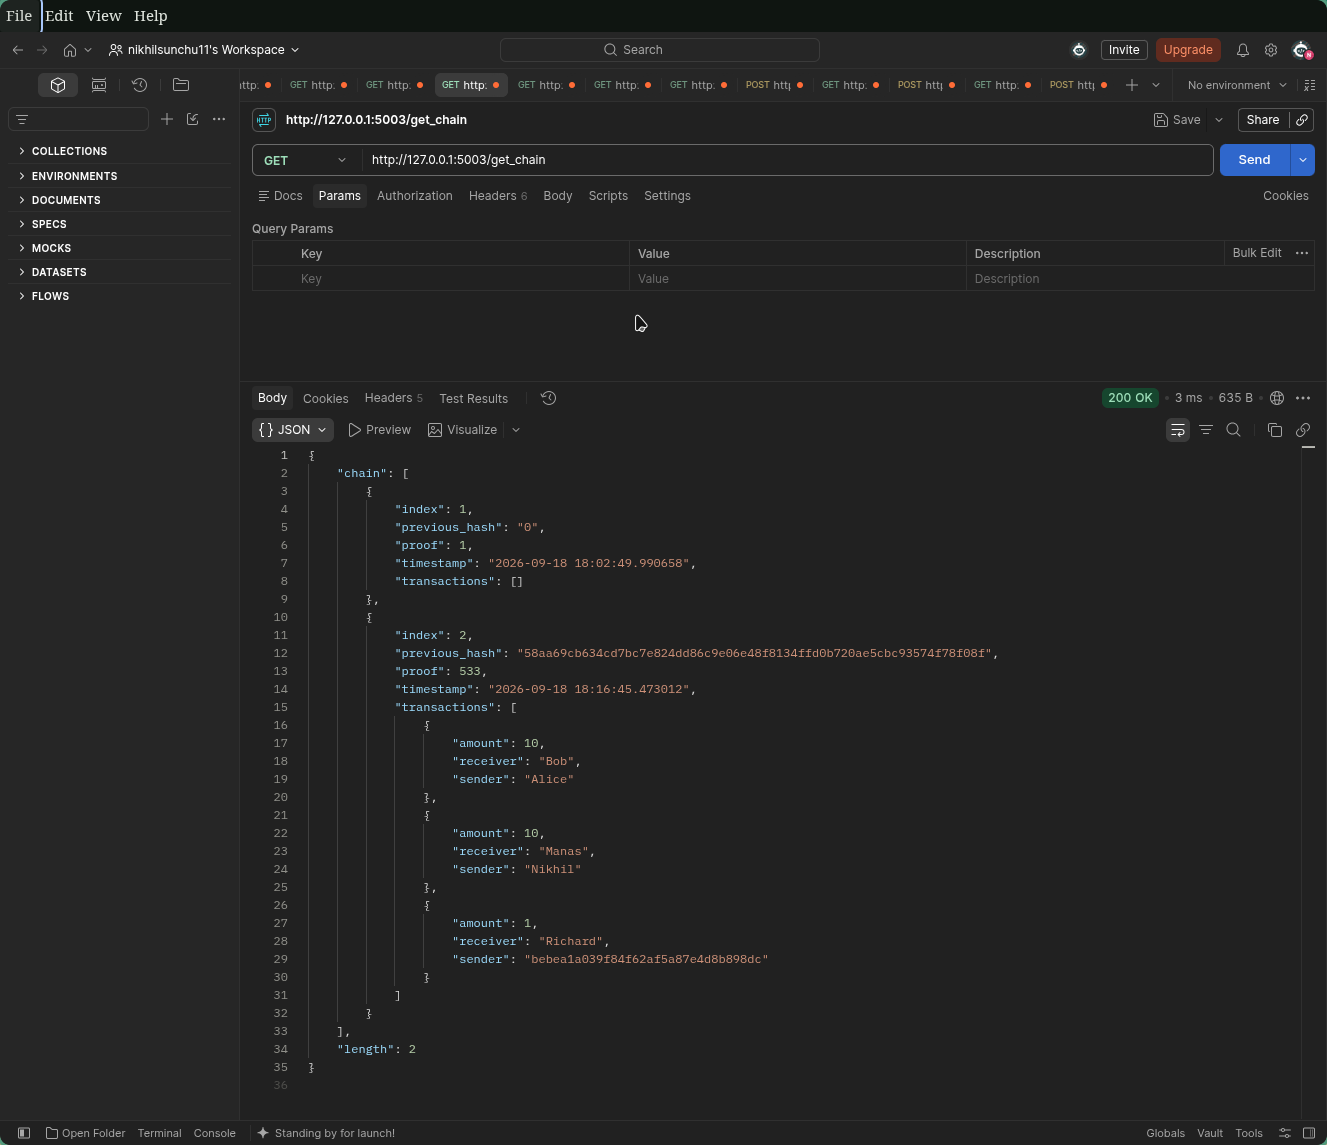
\includegraphics[width=0.58\textwidth]{images/fig13_connect_nodes.png}

{\footnotesize\textbf{Fig. 1} -- Connecting the nodes (POST /connect\_node)}
\end{center}

\subsection{Task 5.1 -- Add Transactions (POST /add\_transaction)}
Transactions were added through a POST request containing the sender, receiver, and amount. \texttt{add\_transaction()} appends the transaction to the pending pool and returns the block index in which it will be mined.

{\renewcommand{\baselinestretch}{0.85}\selectfont
\begin{lstlisting}[style=pythonstyle]
def add_transaction(self, sender, receiver, amount):
    self.transactions.append({'sender': sender,
                              'receiver': receiver,
                              'amount': amount})
    return self.get_previous_block()['index'] + 1

@app.route('/add_transaction', methods=['POST'])
def add_transaction():
    json = request.get_json()
    if not all(key in json for key in ['sender', 'receiver', 'amount']):
        return 'Some elements of the transaction are missing', 400
    index = blockchain.add_transaction(json['sender'],
                                       json['receiver'],
                                       json['amount'])
    return jsonify({'message':
                    f'This transaction will be added to Block {index}'}), 201
\end{lstlisting}
}

\begin{center}
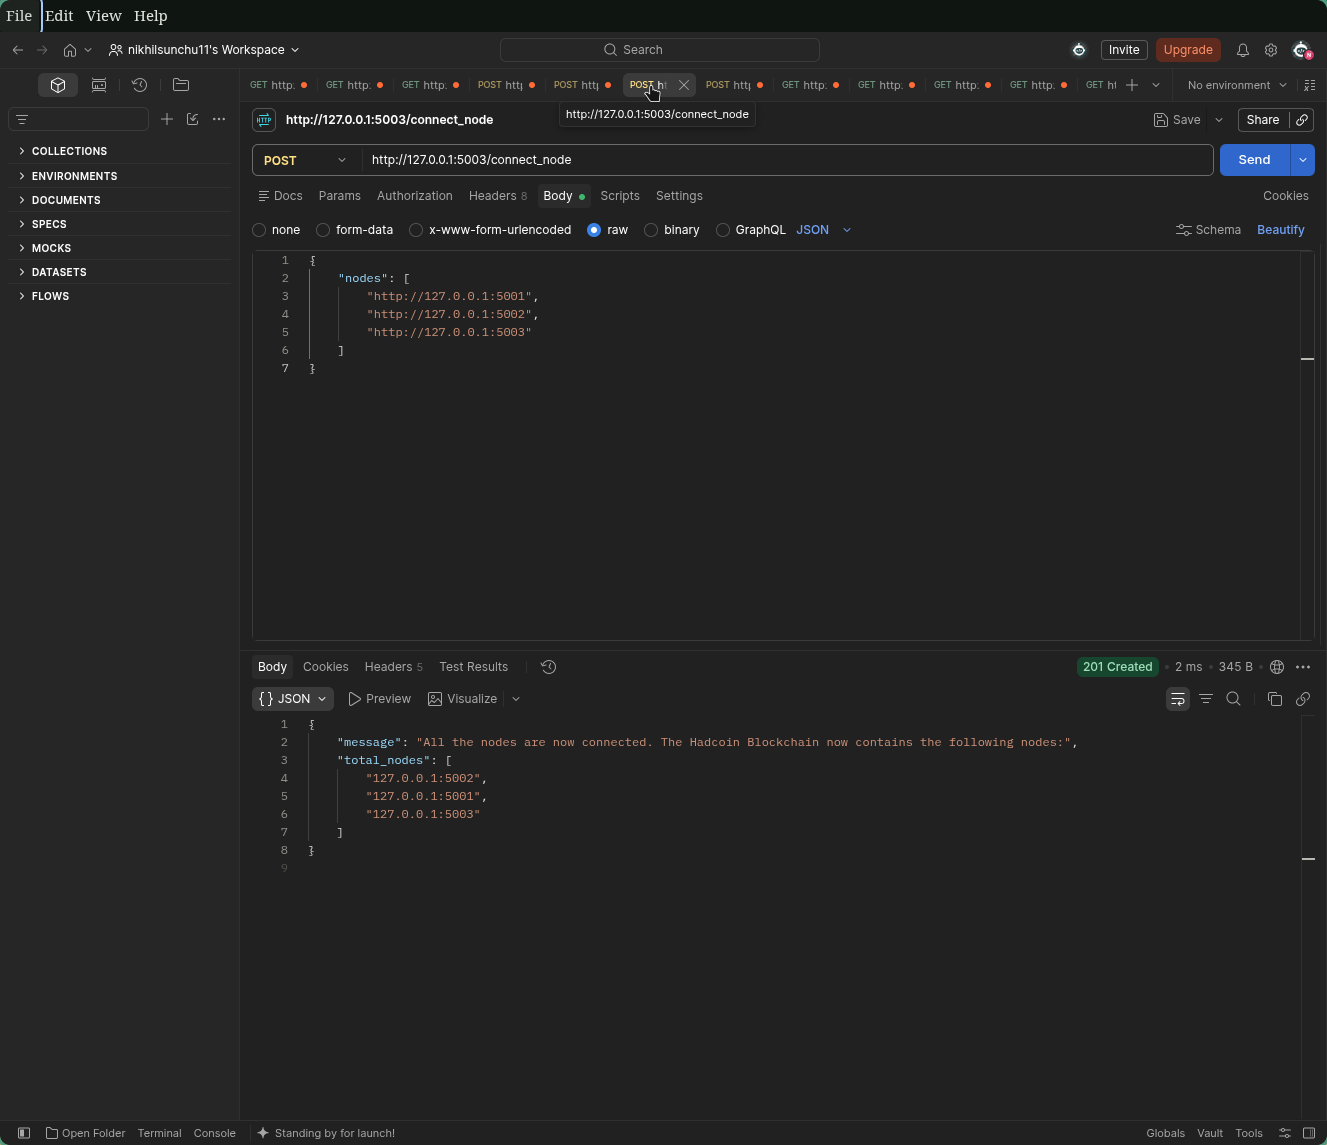
\includegraphics[width=0.58\textwidth]{images/fig6_add_transaction.png}

{\footnotesize\textbf{Fig. 2} -- Adding a transaction (POST /add\_transaction)}
\end{center}

\subsection{Task 5.2 -- Mining (GET /mine\_block)}
Mining was performed with \texttt{mine\_block()}: the node takes the proof of the previous block, solves the Proof-of-Work puzzle (hash starting with \texttt{0000}), and automatically adds a reward transaction of 1 Hadcoin to the miner before creating the block.

{\renewcommand{\baselinestretch}{0.85}\selectfont
\begin{lstlisting}[style=pythonstyle]
@app.route('/mine_block', methods=['GET'])
def mine_block():
    previous_block = blockchain.get_previous_block()
    proof = blockchain.proof_of_work(previous_block['proof'])
    previous_hash = blockchain.hash(previous_block)
    blockchain.add_transaction(sender=node_address,
                               receiver='Richard', amount=1)
    block = blockchain.create_block(proof, previous_hash)
    return jsonify({'message': 'Congratulations, you just mined a block!',
                    'index': block['index'],
                    'timestamp': block['timestamp'],
                    'proof': block['proof'],
                    'previous_hash': block['previous_hash'],
                    'transactions': block['transactions']}), 200
\end{lstlisting}
}

\begin{center}
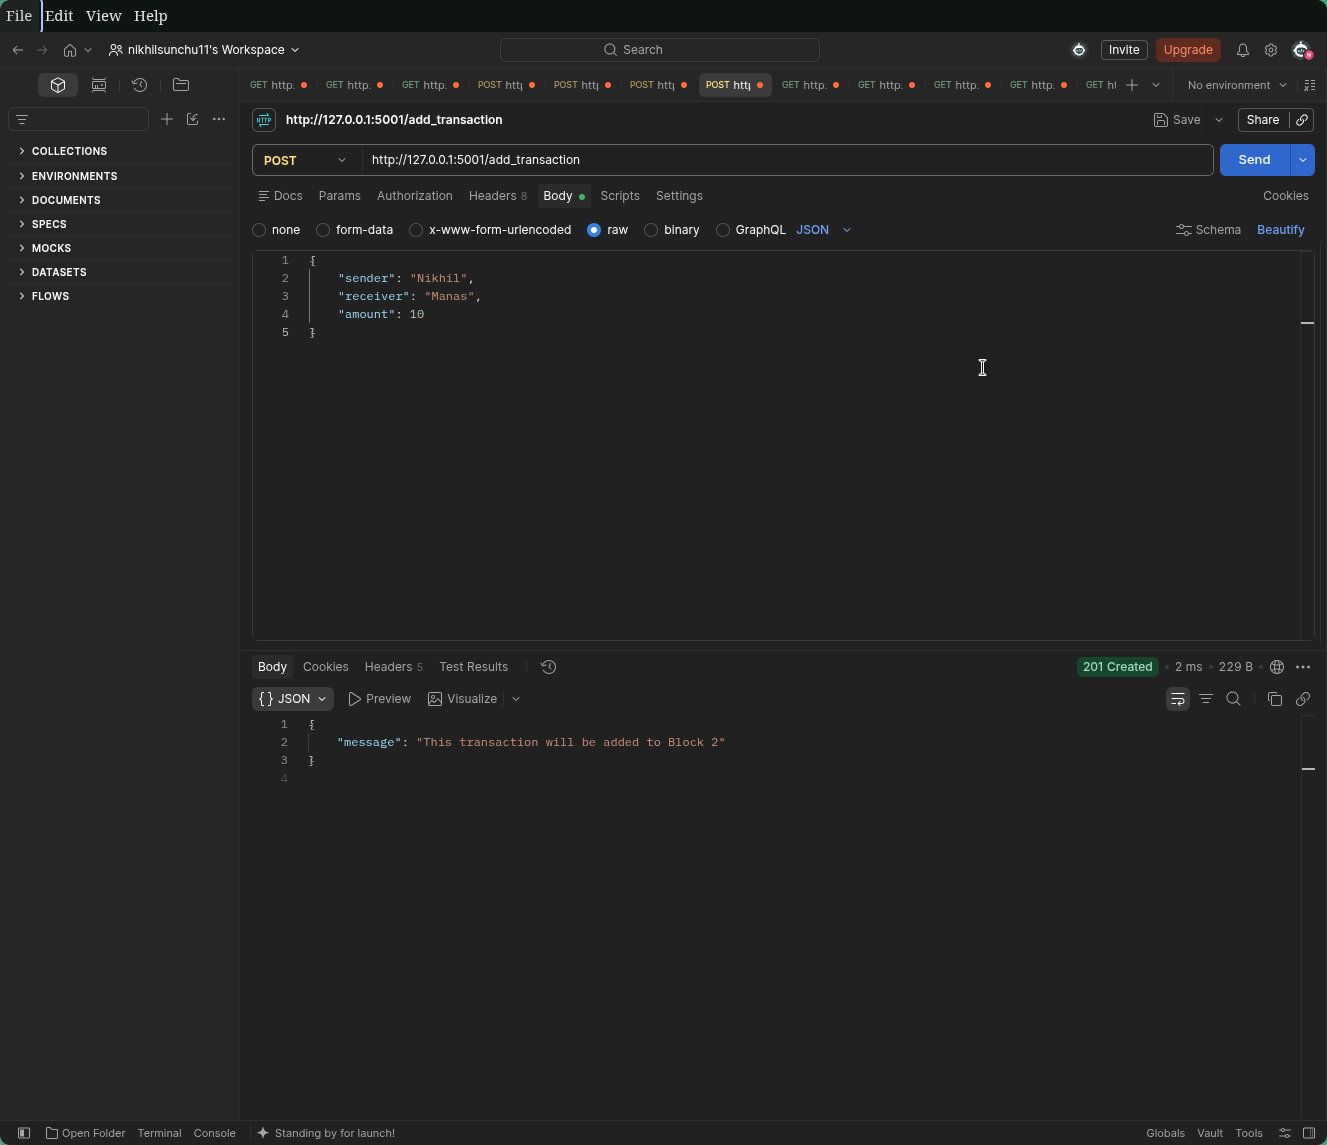
\includegraphics[width=0.58\textwidth]{images/fig7_mine_block_with_tx.png}

{\footnotesize\textbf{Fig. 3} -- Mining a block with the added transaction}
\end{center}

\subsection{Task 5.3 -- Fetch the Chain (GET /get\_chain)}
The complete blockchain of a node was fetched with \texttt{get\_chain()}, which returns the chain together with its length.

{\renewcommand{\baselinestretch}{0.85}\selectfont
\begin{lstlisting}[style=pythonstyle, numbers=none]
@app.route('/get_chain', methods=['GET'])
def get_chain():
    return jsonify({'chain': blockchain.chain,
                    'length': len(blockchain.chain)}), 200
\end{lstlisting}
}

\begin{center}
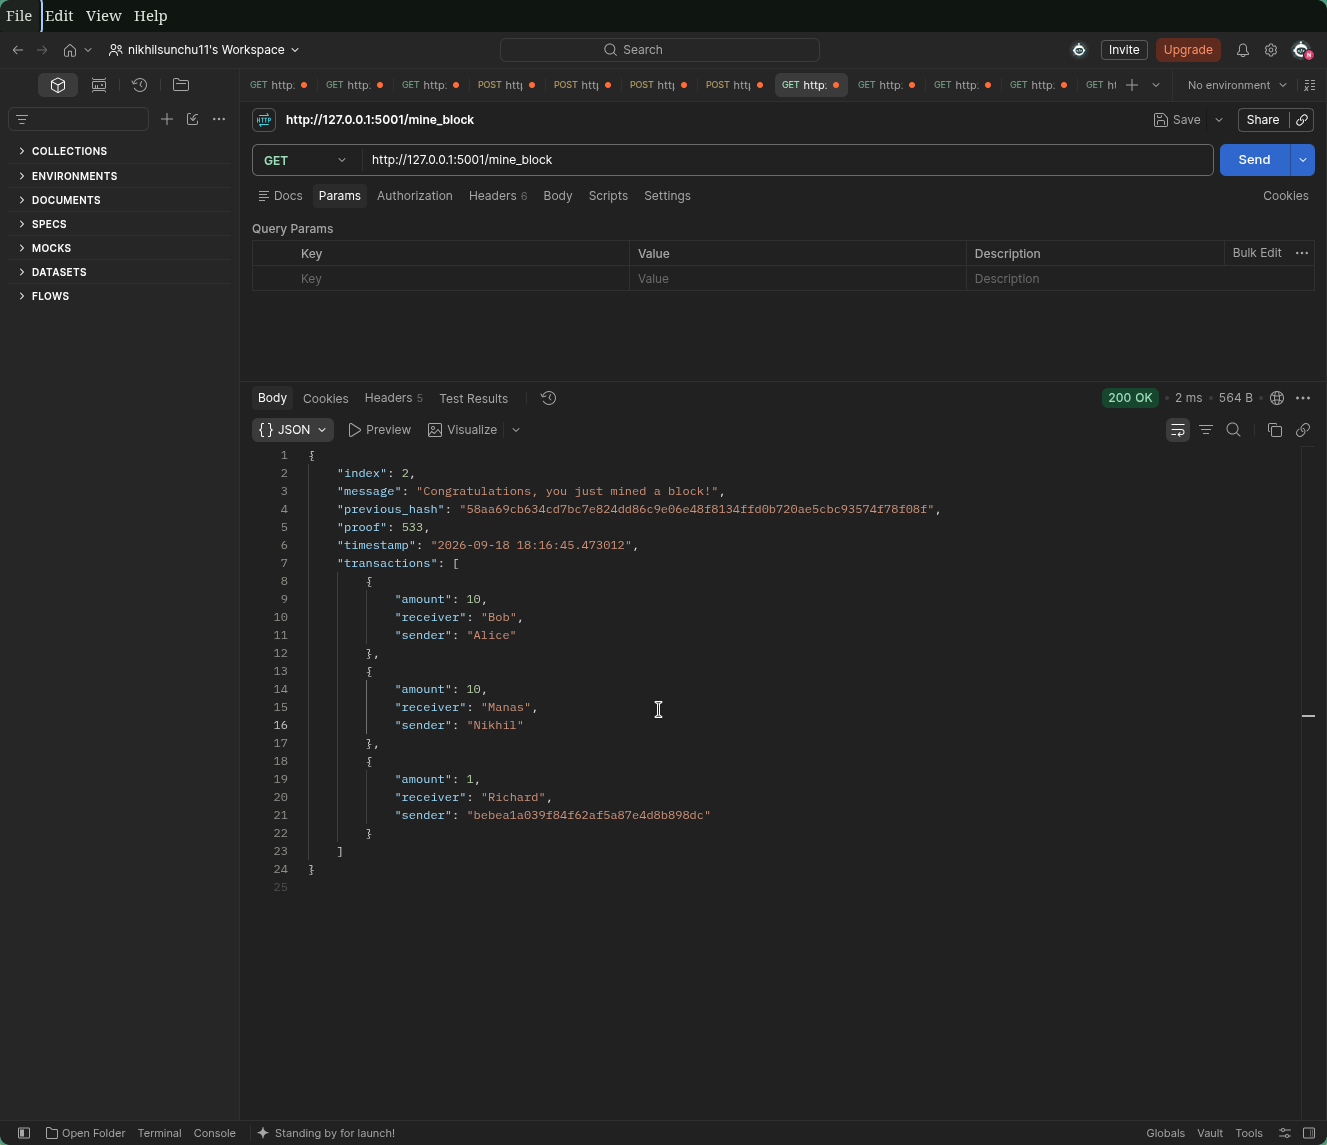
\includegraphics[width=0.58\textwidth]{images/fig8_get_chain_with_tx.png}

{\footnotesize\textbf{Fig. 4} -- Fetching the chain with the mined block}
\end{center}

\subsection{Task 5.4 -- Replace the Longest Chain (GET /replace\_chain)}
After a block was mined on node 5001 while nodes 5002 and 5003 still had only the genesis block, consensus was invoked. \texttt{replace\_chain()} fetches the chain of every registered node and adopts it if it is longer and valid. This was performed on both 5002 and 5003, giving the same result.

{\renewcommand{\baselinestretch}{0.85}\selectfont
\begin{lstlisting}[style=pythonstyle]
def replace_chain(self):
    network = self.nodes
    longest_chain = None
    max_length = len(self.chain)
    for node in network:
        response = requests.get(f'http://{node}/get_chain')
        if response.status_code == 200:
            length = response.json()['length']
            chain = response.json()['chain']
            if length > max_length and self.is_chain_valid(chain):
                max_length = length
                longest_chain = chain
    if longest_chain:
        self.chain = longest_chain
        return True
    return False

@app.route('/replace_chain', methods=['GET'])
def replace_chain():
    replaced = blockchain.replace_chain()
    if replaced:
        return jsonify({'message': 'The chain was replaced by the longest one.',
                        'new_chain': blockchain.chain}), 200
    return jsonify({'message': 'All good. The chain is the largest one.',
                    'actual_chain': blockchain.chain}), 200
\end{lstlisting}
}

\begin{center}
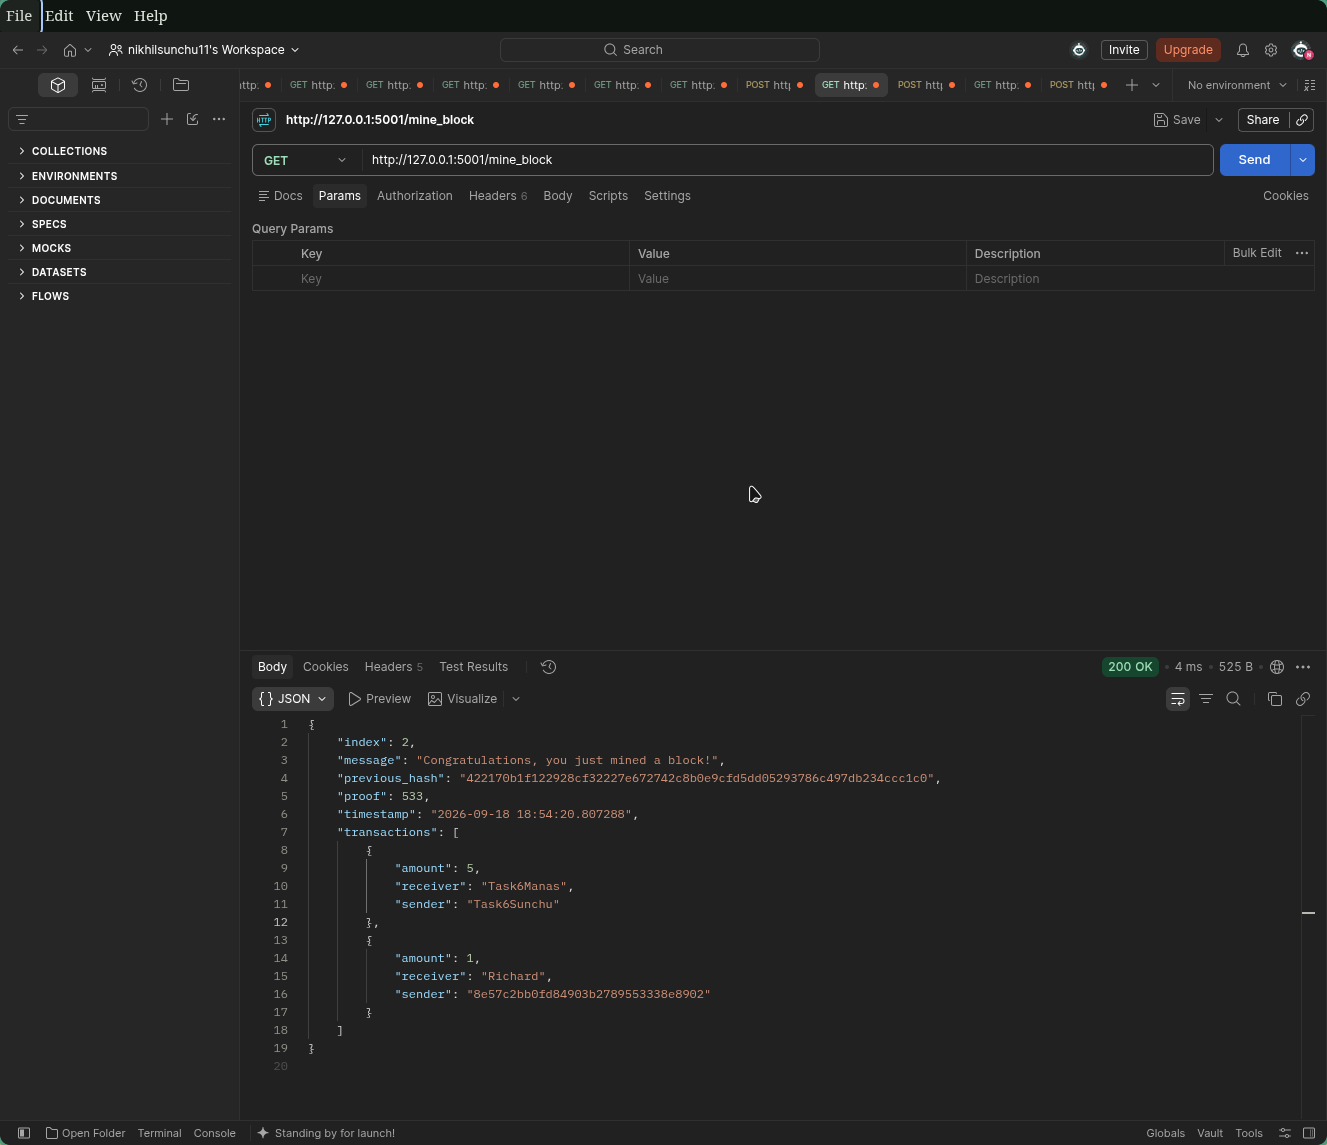
\includegraphics[width=0.58\textwidth]{images/fig18_replace_chain_node5002.png}

{\footnotesize\textbf{Fig. 5} -- Replacing the chain on node 5002; the same result was obtained on node 5003}
\end{center}

\subsection{Task 5.5 -- Final Synchronized Chain}
After the consensus protocol, all nodes converged on the same longest chain, confirming that every node agrees on a single transaction history.

\begin{center}
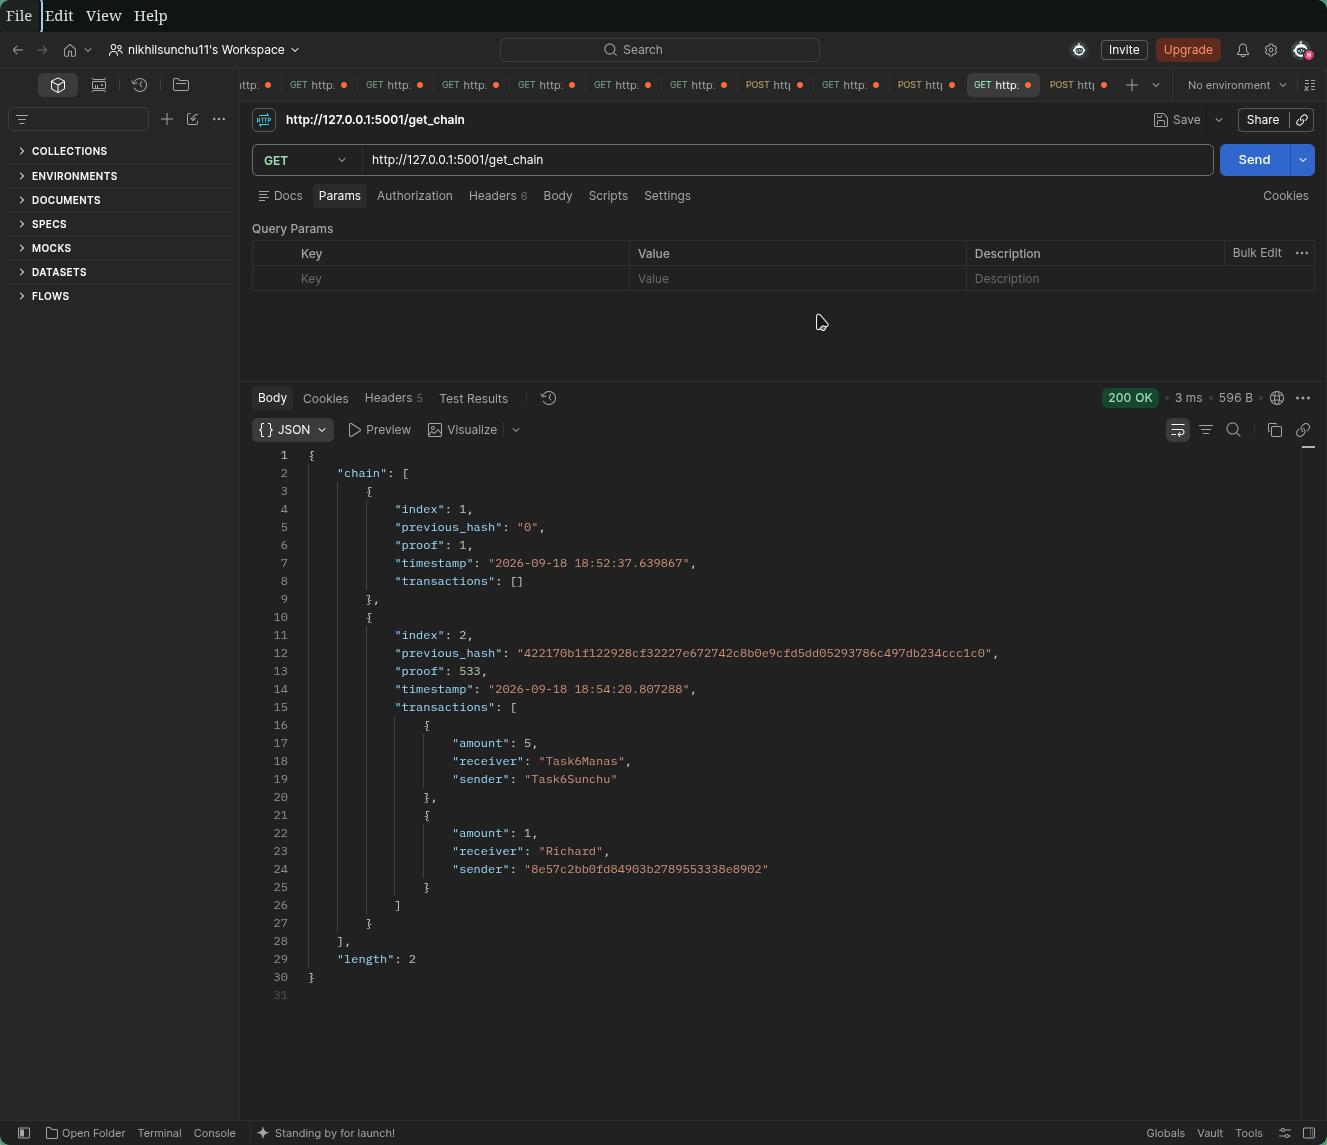
\includegraphics[width=0.58\textwidth]{images/fig20_final_chain_node5001.png}

{\footnotesize\textbf{Fig. 6} -- Final synchronized chain on node 5001}
\end{center}

\subsection{Task 6 -- Remove Transactions After They Are Added to a Block}
The code was modified so that pending transactions are cleared as soon as they are incorporated into a mined block: in \texttt{create\_block()}, the current transaction pool is copied into the block and the pool is then reset, so the same transactions are never mined twice.

{\renewcommand{\baselinestretch}{0.85}\selectfont
\begin{lstlisting}[style=pythonstyle]
def create_block(self, proof, previous_hash):
    block = {'index': len(self.chain) + 1,
             'timestamp': str(datetime.datetime.now()),
             'proof': proof,
             'previous_hash': previous_hash,
             'transactions': self.transactions}
    self.transactions = []      # transactions removed after being added
    self.chain.append(block)
    return block
\end{lstlisting}
}

% -------------------------------------------------
\section{Conclusion}
We developed a cryptocurrency using Python and implemented mining in a simulated three-node blockchain network. Each node maintained its own ledger and synchronized with peers using the Longest Chain Rule to ensure consistency. Mining was performed through Proof-of-Work, securely adding transactions and rewarding miners. This demonstrated key blockchain concepts, including decentralized consensus, transaction validation, and network synchronization.

\end{document}